% #############################################################################
% This is Chapter 4
% !TEX root = ../main.tex
% #############################################################################
% Change the Name of the Chapter i the following line
\fancychapter{Implementation}
\cleardoublepage
% The following line allows to ref this chapter
\label{chap:implementation}

\par In this chapter, implementation of Direct methods based in the usage of Bernstein Polynomails are used in both Matlab and Python will be discussed. This chapter focuses on formalising the optimisation problem for multipe vehicles. Given that a Direct Method is used, once the optimisation problem is formalised, it can be solved by a whole range of non linear optimisation algorithms.

\section{The Optimisation Problem}

\par The Motion Planning problem for multiple vehicles that will be focused for the project consists in a go-to formation manoeuvre \cite{sabetghadam2018cooperative}. The go-to formation manoeuvre consists of the simultaneous arrival of a formation of vehicles to desired locations whilst simultaneously avoiding collisions between each other and the environment.

\par Just as for the case of optimisation for a single vehicle, motion planning for multiple vehicles will also be based on the minimisation of an appropriate cost function. This time, however, the cost will be the result of the sum of the costs of each individual vehicle and an added constraint will be necessary that will take into account inter vehicle collisions. 

\par The optimal control problem can be redefined for multiple vehicles as 
\begin{equation}
    \label{eq:multi_cost}
    \begin{aligned}
    & \underset{x^{[i]}(.),u^{[i]}(.),i= 1,\dots N_v}{\text{minimize}} && \int_0^T \sum_{i=1}^{N_v}  L_i (x^{[i]}(t),u^{[i]}(t))dt + \Psi (x(T)) \\
    & \text{subject to}  && x^{[i]}(0) = x_0^{[i]}, \\
        & && x^{[i]}(T) = x_f^{[i]}, \\
        & && \dot{x}^{[i]} = f_i (x^{[i]}(t), u^{[i]}(t)), &&& t \in [0,T]\\
        & && c_{col} (x^{[i]},u^{[i]} ) \geq 0, \\
        & && h(x(t),u(t)) \geq 0, \\
        & && \underline{x}^{[i]} \leq x^{[i]} (t) \leq \overline{x}^{[i]} , \\
        & && \underline{u}^{[i]} \leq u^{[i]} (t) \leq \overline{u}^{[i]}
    \end{aligned}
\end{equation}

\par This problem will also produce a solution within time horizon $T$. Initial and terminal constraints will exist for every vehicle, as well as inter-vehicle constraints.

\par A problem that only has the integral term $\sum_{v=1}^{N_v} L_v(x^{(v)}(t),u^{(v)}(t))$ is said to be in \textit{Lagrange form}, a problem that optimises only the boundary objective $\sum_{v=1}^{N_v} \Psi_v(x(T))$ is said to be in \textit{Mayer form} and a problem with both terms is said to be in \textit{Bolza form}. An example where only the \text{Mayer form} would be necessary could be a situation where the desired destination of the vehicles does not have enough room for them all to be arranged in their desired positions. Therefore, the goal of the optimiser is to find the closest to the desired positions.

\section{The Log Barrier Function}

\par A log barrier functional can be added to the cost functional such that the motion planning problem becomes unconstrained. Specifically, the inequality constraints are moved into the cost functional by applying a log barrier funcional to them.
\par An optimisation problem of the form 
\begin{equation}
    \label{eq:opt_prob_without_log_bar}
    \begin{aligned}
    & \text{minimize} && \int_0^T l(x(\tau),u(\tau),\tau)d\tau + m(x(T)) \\
    & \text{subject to}  && \dot{x}(t) = f(x(t)),u(t),t),\quad x(0)=x_0 \\
        & && c_j(x(t)),u(t),t)\leq 0, \qquad t\in [0,T],j\in \{1,\dots,k \}
    \end{aligned}
\end{equation}
becomes
\begin{equation}
    \label{eq:opt_prob_with_log_bar}
    \begin{aligned}
    & \text{minimize} && \int_0^T l(x(\tau),u(\tau),\tau)+\sum_j \beta_\delta(-c_j(x(t),u(t),t))d\tau + m(x(T)) \\
    & \text{subject to}  && \dot{x}(t) = f(x(t)),u(t),t),\quad x(0)=x_0 \\
    \end{aligned}
\end{equation}

where $\beta_\delta(\cdot)$ is a function that is steep in infeasible solutions and nearly constant in feasible solutions. Given that the inequality constraint functionals must be negative for the solution to be feasible, $\beta_\delta(-c_j(\cdot))$ must be nearly constant for positive values. One possible log barrier functional can be
\begin{equation}
    \beta_\delta (z) = 
    \begin{cases}
        -\log{} z & z>\delta \\
        \frac{k-1}{k}\left[\left(\frac{z-k\delta}{(k-1)\delta}\right)^k-1\right]-\log{}\delta & z\leq \delta
    \end{cases}
\end{equation}
which is continuous and whose derivative around $z=\delta$ is continuous too. For full reference see \cite{hauser2006barrie}.
\par The "hockey stick" function, with form
\begin{equation}
    \delta(z)= \begin{cases}
        \tanh(z), & z\leq 0 \\
        z, & z<0
    \end{cases}
\end{equation}
can be applied to the log barrier functional such that its derivative is smaller for feasible solutions. Figure \todo{plot the log barrier with and without the hockey function (hausler page 110)} shows the log barrier function with and without the hockey function applied.

\section{Inter-Vehicular Constraints}

\par There are 2 ways of preventing inter-vehicle collision; \textit{spatial deconfliction} and \textit{temporal deconfliction} \cite{hausler2015mission}.
Spatial deconfliction is appropriate for \ac{PF} and imposes the constraint that the spatial paths of the vehicles under consideration will never intersect and keep a desired safe distance from each other. Temporal deconfliction is appropriate for \ac{TT} and requires that two vehicles will never be ”at the same place at the same time”. However, their spatial paths are allowed to intersect. Figure \ref{fig:deconfliction} illustrates the two types of deconfliction strategies. Temporal deconfliction allows an extra degree of freedom and will intuitively lead to cheaper dynamic costs.

\begin{figure}
    \centering
    \begin{subfigure}[b]{0.45\textwidth}
        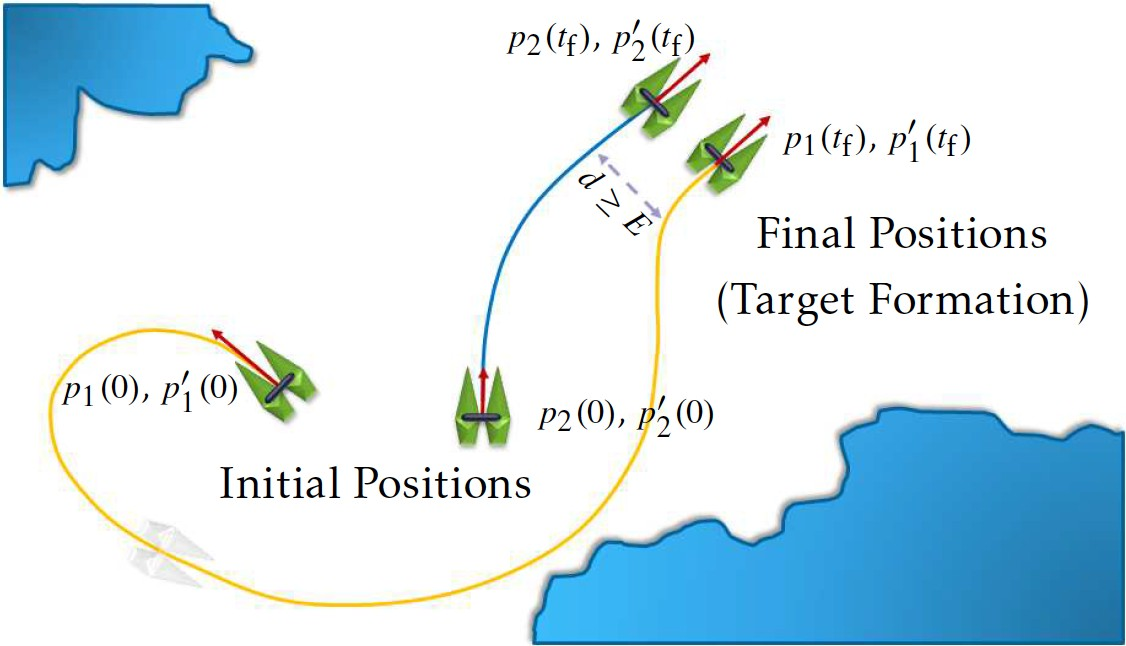
\includegraphics[width=\textwidth]{Images/spacial_deconf.jpg}
        \caption{Spacial Deconfliction}
    \end{subfigure}
    ~
    \begin{subfigure}[b]{0.45\textwidth}
        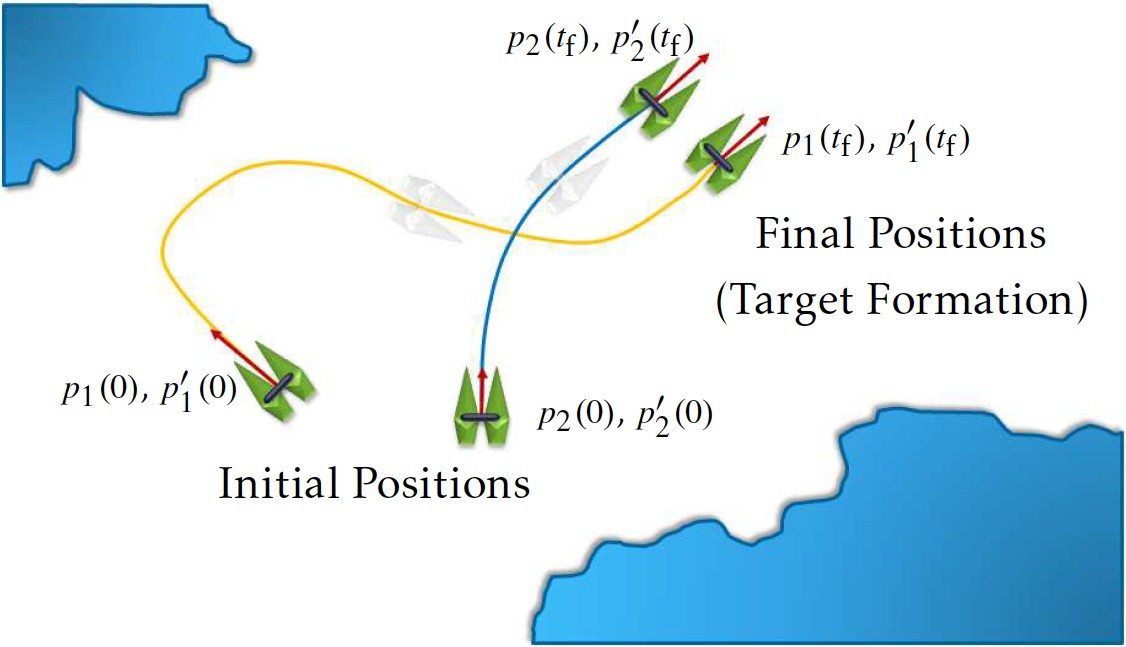
\includegraphics[width=\textwidth]{Images/temporal_deconf.jpg}
        \caption{Temporal Deconfliction}
    \end{subfigure}
    \caption{Inter Vehicle deconfliction Solutions}
    \label{fig:deconfliction}
\end{figure}

\par Two method for temporal deconfliction were implemented, one based on sampling the curves and the other based on directily exploiting the properties of Bezier Curves.

\par For $N_v$ vehicles, any of ${N_v \choose 2}$ pairs could lead to a collision, therefor, all pairs must be tested, which means a quadratic complexity, therefor, finding fast algorithms to calculate the distance between each pair of trajectories becomes essential.
\par The easiest method of guaranteeing that the minimum distance between a pair of vehicles is always above a certain value is by calculating the minimum possible distance between each pair of $N_v$ vehicles, which yields a total of ${N_v \choose 2}$ calculations. If \ac{PF} is used, then the minimum distance between the paths must be greated than a certain value. As a result, these paths cannot intersect. If \ac{TT} is used, then the minimum distance between vehilces will depend on time $t \in [0 T]$, which means that the trajectories must intersect in space but not in time. 

\subsection{Sampling Trajectories}

\par Given that this thesis will focus on the usage of \ac{TT} and not \ac{PF}, methods to calculate minimum distances throughout time will be discussed, i.e., minimum distance between trajectories.
\par The most straightforward way to calculate the minimum distance between two trajectories is to sample each trajectory and calculate the euclidean distance between time equivalent samples. The smallest yields the shortest distance. This method, however, is not perfect because the finer the samples, the more accurate is the result. 
\par One thing to note, however, is that super accurate results of minimum distance between trajectories are not necessary. If, besides knowing the position of the vehicle at a sample, we also know the maximum tangent speed between that sample and the next, then the distance to the other vehicle cannot deviate more than a certain determinable value between those 2 points. It will be smaller than the calculated distance if the vehicles are moving towards eachother. The choice of number of samples will determine how big this deviation can be. The opitmisation algorithm will stop once it finds a minimum distance that is greater than a certain value, therefor, the number of samples must be big enough such that the deviation is relatively small when compared to the desired minimum distance. 
\par For example, an optimisation problem specifies a minimum distance between 2 vehicles of \SI{1}{\meter}. These vehicles are limited to \SI{1}{\meter\per\second}. At a certain point in time between 2 samples, they can be closer to eachother than they are at the samples, so lets assume the worst case scenerio: half of the time between samples is spent moving towards eachother at maximum speed, which imples moving away from eachother during the other half of time at maximum speed, therefor, if the time sample is \SI{10}{\milli\second}, during \SI{5}{\milli\second} the vehicles can travel \SI{1}{\centi\meter} towards eachother, at the relative speed of \SI{2}{\meter\per\second}, which is a \SI{1}{\percent} deviation from the established minimum distance of \SI{1}{\meter}. If the optimisation problem is reformulated to guranatee \SI{1.01}{\meter}, then, with samples spaced by \SI{10}{\milli\second}, a successful optimisation solution guarantees a minimum distance between vehicles of \SI{1}{\meter}. which means a total of 100 samples per second of runtime.


\subsection{Bezier Curve to a point}
\label{sec:bezcurvetopoint}

\par The next method is based on calculating the minimum distance between Bezier curves \cite{chang2011computation}. This algorithm is addapted to calculate the minimum distance between a curve and a polygon. By subtracting one trajectory to another, which for Bezier curves is explained in section \ref{sec:bezcurves}, finding the minimum distance between trajectories gets translated to finding the closest point of this subtraction curve to the origin. The origin can be interpreted as a 1 point convex shape, therefor, what follows is a brief explanation of an iterative algorithm to calculate the minimum distance of a Bezier curve to a polygon, which will also be used to do collision avoidance with arbitrary convex shapes.

\par This algorithm consists in recursively breaking down the trajectory into halves by obtaining a new set of control point for each half via de deCasteljau algorithm. For each half, two values are calculated: an upper bound of the minimum distance and a lower bound. The upper bound for the minimum distance will be the closest endpoint of the segment to the polygon, a lower bound is the closest point of the convex hull of the new control points to the polygon. The exit condition of the recursion is when the lower bound is relatively small when compared to the upper bound. The lower bound may be zero if the shapes intersect, which has no influence on the execution of the algorithm. If the exit condition isn't met, the recursion is repeated and the returned value is the smallest of the upper bound along with the time at which the smallest value was found.

\subsection{GJK Algorithm}
\label{sec:gjkalg}

\par The \ac{GJK} algorithm is a necessary tool for calculating the minimum distance between a Bezier Cuve and a point or polygon, therefor, it is explained here.

\par The \ac{GJK} algorithm is an effitiend algorithm to calculate minimum distance between arbitrary convex shapes in any dimension. 
\par The \ac{GJK} algorithm relies heavily on a concept called the Minkowski Sum, but, because the difference operator is used for this algorithm, instead of the sum, the term Minkowski difference will be used. For two shapes $A$ and $B$, their Minkowski Difference is given by
\begin{equation}
    D = A - B = \{a-b|a\in A, b\in B\}
\end{equation}
where $D$ is a new convex shape given by the subtraction of every point in $A$ by every point in $B$.
Figure \todo{figure of 2 intersecting shapes plus figure } shows 2 shapes on the left handside which intersect and the resulting Minkowski Difference on the right hand side. Figure shows two shapes that do not intersect and their resulting Minkowski Difference. Notice how the second Minkowski Difference has an identical shape to the first, only differing on its position.
If the Minkowski Difference contains the origin, then the two shapes have common points, i.e., intersect, because the resulting subtraction is zero. As a result, the \ac{GJK} algorithm is a two part problem: first detect intersection, by testing if the Minkowski Difference contains the origin, then, if it does not, the closest points between $A$ and $B$ result in a Minkowski Point that is closest to the origin, therefor, the second part part of the problem is to look for that closest point to the origin.
\par For a N-D Minkowski Difference, if a convex shape of up to N+1 vertices that surrounds the origin is found, then the shapes $A$ and $B$ intersect. This shape with up to N+1 vertices is known as a simplex. For 2-D Minkowski Differences, the simplexes can be a point (1 vertex), a line segment (2 vertices) and a triangle (3 vertices). For 3-D spaces, the simplexes can be the same as in 2-D spaces with the addition of a tetrahedron (4 vertices).
\par The key to \ac{GJK}'s effitiency is to find points in the Minkowski difference that are the best candidates to be in a simplex that can contain the origin. 
\par A support function returns the farthest point in some direction. The resulting point is known as the support point. Finding a support point in the Minkowski Difference along direction $d$ is the same as subtracting the support point of $A$ along $d$ and $B$ along $d$. 
\par Choosing the farthest point in a direction has significance because it creates a simplex who contains a maximum area therefore increasing the chance that the algorithm exits quickly. In addition, all the points returned this way are on the edge of the Minkowski Difference and therefore if a point past the origin along some direction cannot be added, the Minkowski Difference cannot contain the origin. This increases the chances of the algorithm exiting quickly in non-intersection cases.

\par Let $W_k$ be the set of vertices of the simplex constructed in the $k^{th}$ iteration, and $v_k$ as the point in the simplex closest to the origin. Initially, $W_0=\varnothing$, and $v_0$ is an arbitrary point of the Minkowski Difference. Since each $v_k$ is contained in the Minkowski Difference, the length of $v_k$ must be an upper bound for the distance.
\par \ac{GJK} generates a sequence of simplices in the following way. In each iteration step, a vertex $w_k = s_{A-B}(-v_k)$ is added to the simplex, with the objective of surrounding the origin. If the simplex contains the origin, then the program interrupts because the shapes intersect. If it's proven that the Minkowski Difference cannot contain the origin because the last added vertex did not move "beyond" the origin, then program interrupts and moves on to finding the minimum distance to the origin. If intersection is not proven yet, the new $v_{k+1}$ is perpendicular to the vector given by the last vertex with the one before that, or with the last with the third from the last, if availabe, depending on which has a dot product greater than 0, and the not used vertex gets removed from the simplpex. Alternatively, if no intersection is proven, the new $v_{k+1}$ is the point in the convex hull of $W_k\cup \{w_k\}$ closest to the origin and $W_{k+1}$ becomes the smallest sub-simplex of $W_k\cup \{w_k\}$ that contains $v_{k+1}$.


\section{Minimum Distance to Convex Shapes}

\par Earlier, in section \ref{sec:bezcurvetopoint}, an algorithm to calculate the distance of a trajectory to a polygon was presented. This algorithm, however, is limited to polygons that do not intersect with the trajectory. If the curve intersects with the convex shape, the algorithm returns zero as minimum distance. Optimisation algorithms, like Sequential Quadratic Programming, require the derivative of the constraints to be non zero, even when the current guess for solution is not feasible because this derivate, in other words, will "inform" how far the control points must move so that the solution becomes feasible.

\par A modification to the algorithm that calculates the minimum distance to a convex shape is presented to calculate the intersection points between the curve and the shape. Aftwards, these intersection points are used to calculate a "penetration" of the curve in the shape.
\par First thing to note is, during the recusion of the minimum distance algorithm, some endpoints of the cut segments will land inside the shape. If a segment has an endpoint inside and an endpoint outside the shape and the distance between these two points is approximately zero, then the point inside is added to a stack of intersecting points, otherwise, the recursion continues. If the control points of the recursive segments are partially in the shape while others are not, then the recursion continues, otherwise, if the control points are all outside or all inside the shape, then there is no point in continuing because the segment cannot contain anymore intersection points.
% \par One thing that can be pointed out that can speed up checking if all of the control points of a segment are contained in the shape or not is by finding the convex hull of of the shape. If some control points are on the convex hull. The advantage of this way of testing if all control points are in the shape is that the complexity of the convex hull algorithm, will be $\mathcal{O}(n\log{}n)$, 
\par Once the intersection points are found, the "penetration" must be calculated. This consists first in finding a convex hull that intersects the shapes. If the number of intersection points is two, then the deCasteljau algorithm is performed twice to find a set of control points for the segment that starts and ends with these two points and the convex hull of these control points is taken, otherwise, the convex hull of all of the intersecting points is used. Once the convex hull is determined, the \ac{DEPA} algorithm explained in section \ref{sec:epaalg}  is performed with the obstacle shape along a predifined direction $d$. The bigger the penetration depth, the more the trajectory is "deeper" in the curve.



\subsection{Directed EPA}
\label{sec:epaalg}

% https://graphics.stanford.edu/courses/cs468-01-fall/Papers/van-den-bergen.pdf

\par If two convex shapes intersect, the \ac{GJK} algorithm cannot provide collision information like the penetration depth and vector. One algorithm that provides this information is the \ac{EPA}.
A slight modification for the \ac{EPA} algorithm is proposed here. It will be refered as the \ac{DEPA}, whose objective is to find the penetration of one convex shape relative to another along a specific direction $d$, while the \ac{EPA} algorithm finds the shortest vector such that the shapes no longer collide. The penetration along a direction is the length of dislocation that the second shape would have to move so that the two shapes no longer collide. 
\par The shapes intersect when the Minkowski contains the origin, therefor, the \ac{EPA} or the slight variant shown here have as objective dislocating the Minkowski Difference such that it no longer contains the origin. Penetration along a specific direction can be found by calculating the length of the vector that starts in the origin on the Minkowski Difference, has the same direction as $d$, and stops once it finds the edge of the Minkowski Difference. In other words, this is the norm of the intersection point between a ray starting at the origin with direction $d$ and the edge of the Minkowski Difference. Once this length is found, shape $B$ can move by that length along the direction of $d$ such that it is no longer in collision with shape $A$.
\par The process of looking for the penetration along a direction $d$ starts with a polygon which contains the origin, constructed with points along the edge of the Difference. The first step is to find the only edge of this polygon with will intersect with the ray that starts in the orgin with direction $d$. Once this edge is found, the other edges of the polygon are ignored and an interative process starts. The first step on the iterative process is to calculate a vector which normal to the current intersecting segment and points "outwards" with respect to the origin. Next, the support function is performed with this vector. The resuting point will be closer to the desired final point. There are now three points in play: the two segment ends and the new point that resulted from the support operation. The next step is to define two segments, one from the one of the segment ends to the new support point, the other from the other segment end to the support point. The next step is to find which of these two new segments intersects with the same ray with direction $d$ and then repeat the iteration. 



\section{Description of the implemented code}

\par The variables for the motion planning problem are each vehicle's state variables and inputs, as explained in chapter \label{chap:autonomousvehiclemodels}. Each of these variables will be refered to as curves. Optimisation algorithms cannot take continuous functions as variables, therefor, some form of parameterisation of each curve is necessary, as exemplified in some of the algorithms of chapter \label{chap:theory}. Here, each curve will be represetend as a Bernstein Polynomial with order $N$, which will require $N+1$ control points. A destinction is made between state variables and inputs: state variables must have establised initial and final conditions, inputs do not. This implies that for state variables, the initial and final control points must be fixed, therefor, they do not need to participate on the optimisation problem. The following matrix represents how the control points are stored so that they can be accessed by all functions that perfom operations on the curves

\begin{equation}
    \begin{bmatrix}
        \colorbox{yellow}{$\displaystyle x_0^0$} & \colorbox{yellow}{$\displaystyle y_0^0$} & \colorbox{yellow}{$\displaystyle \psi_0^0$} & \colorbox{yellow}{$\displaystyle u_0^0$} & \colorbox{yellow}{$\displaystyle v_0^0$} & \colorbox{yellow}{$\displaystyle r_0^0$} & \tau_{u_0}^0 & \tau_{r_0}^0 \\
        x_1^0 & y_1^0 & \psi_1^0 & u_1^0 & v_1^0 & r_1^0 & \tau_{u_1}^0 & \tau_{r_1}^0 \\
        \vdots & \vdots & \vdots & \vdots & \vdots & \vdots & \vdots & \vdots \\
        \colorbox{yellow}{$x_{N}^0$} & \colorbox{yellow}{$y_{N}^0$} & \colorbox{yellow}{$\psi_{N}^0$} & \colorbox{yellow}{$u_{N}^0$} & \colorbox{yellow}{$v_{N}^0$} & \colorbox{yellow}{$r_{N}^0$} & \tau_{u_{N}}^0 & \tau_{r_{N}}^0
    \end{bmatrix}
    \label{eq:matrixofvariables}
\end{equation}

\par It is believed \todo{can this be said? because I'm not referencing anything (I'm taking Venanzio's word for it)} that \texttt{fmincon()} performs better when all variables are stored in a line vector, therefor, a function called \texttt{matrify()} is necessary in order to transform the flattened optimisation variable to the matrix of equation (\ref{eq:matrixofvariables}). 
\par Elements marked in yellow do not participate in the optimisation algorithm. They are concatenated to this matrix in \texttt{matrify()}. 

\par High orders are preferable for each curve \cite{cichella2018bernstein} because the higher the curve, the closer the control points are to the "matching" point in time of the curve, which is achieved once an optimisation problem finishes. Chapter \ref{chap:results} exemplifies show the control points approximate to the curve and how it is advantageous to produce the dynamics.

\par A more precise way to calculate the minimum distance of a Bezier curve to a point or to another curve, compared to the one implemented on section \ref{sec:2_d_bezier} is via the algorithm presented in \cite{chang2011computation}. This algorithm takes into account the convex hull property of Bezier Curves and the \textit{deCasteljau} algorithm for subdividing curves. It will also employ the GJK algorithm, a fast and efficient way of calculating distances between 2 convex shapes\cite{cichella2018bernstein}.
\par The fast calculation of distances between these curves allows Bezeir Curves to be appropriate for testing non-linear constraints in multiple vehicle motion planning optimisation.

\par This fancy algorithm performed poorly because it was iterative. A simpler way to calculate the minimum distance was necessary. This consited in subtracting each pair of 2-D curves for each vehicle to eachother, then getting a rough guess of the closest point of that resulting curve to 0: by performing degree elevation to an order 10 times the original then looking for the closest point to the origin. 

\par Minimum distance of the curves to objects was done with GJK. but it was slow

\par Collision to circles is calculated by subtracting the 2-D curve tto the centre of the circle, performing degree elevation of the resultign curve, calculating the closest to the origin and checking wether that distance is greater to the radius. Performing the check for every control point was also done but wasn't advantageous (slower runtime), the reason could be because the derivative of each of these distances or the elevated curve with respect to the position of the control points depends on more than 1 control points of the non elevated curve, therefor, some computation is redundant.


\par The optimisation problem is formulated by constructing a data structure with the fields of table \ref{tab:constants_description}. In Python the same fields are necessary, however, they must be stored in a python dictonary. 


\begin{table}[]
\centering
\begin{tabular}{|l|l|l|l|}
\hline
\textbf{field} & \textbf{description} & \textbf{mandatory} & \textbf{example} \\ \hline
\texttt{T} & Time horizon & yes & \texttt{10} \\ \hline
\texttt{xi} & initial conditions & yes & \texttt{[0 0 0 1 0]} \\ \hline
\texttt{xf} & final conditions & yes & \texttt{[5 5 pi/2 1 0]} \\ \hline
\texttt{N} & order of the curves & yes & \texttt{15} \\ \hline
\texttt{obstacles} & polygons & \begin{tabular}[c]{@{}l@{}}no\\ default: \texttt{[]}\end{tabular} &  \\ \hline
\texttt{obstacles\_circles} & circles & \begin{tabular}[c]{@{}l@{}}no\\ default: \texttt{[]}\end{tabular} &  \\ \hline
\texttt{min\_dist\_int\_veh} & \begin{tabular}[c]{@{}l@{}}minimum distance between \\ vehicles for every point in time\end{tabular} & \begin{tabular}[c]{@{}l@{}}no\\ default: \texttt{0}\end{tabular} & \texttt{.8} \\ \hline
\texttt{numinputs} & \begin{tabular}[c]{@{}l@{}}number of input variables\\ (don't have initial conditions)\end{tabular} & \begin{tabular}[c]{@{}l@{}}no\\ default: \texttt{0}\end{tabular} &  \\ \hline
\texttt{uselogbar} & \begin{tabular}[c]{@{}l@{}}make the problem completely \\ unconstrained and use log \\ barrier functionals\end{tabular} & \begin{tabular}[c]{@{}l@{}}no\\ default: \texttt{false}\end{tabular} &  \\ \hline
\texttt{usesigma} & \begin{tabular}[c]{@{}l@{}}a boolean for the usage of the \\ sigma function if log barrier \\ functionals are to be used\end{tabular} & \begin{tabular}[c]{@{}l@{}}no\\ default: \texttt{false}\end{tabular} &  \\ \hline
\texttt{costfun\_single} & \begin{tabular}[c]{@{}l@{}}a function used to calculate \\ the running cost for each \\ singular vehicle\end{tabular} & yes & \texttt{@costfun} \\ \hline
\texttt{dynamics} & \begin{tabular}[c]{@{}l@{}}a function that describes how the \\ non linear dynamics of the state \\ variables and inputs are linked\end{tabular} & yes & \texttt{@dynamics} \\ \hline
\texttt{init\_guess} & \begin{tabular}[c]{@{}l@{}}a function that provides an initial \\ guess for the optimisation problem \\ which may  speed up the process \\ of optimisation\end{tabular} & \begin{tabular}[c]{@{}l@{}}no \\ default:\\ \texttt{@rand\_init\_guess}\end{tabular} & \texttt{@init\_guess} \\ \hline
\texttt{recoverxy} & \begin{tabular}[c]{@{}l@{}}a function that returns the x and y\\ variables by solving just the initial \\ value problem of the inputs\end{tabular} & yes & \texttt{@recoverxy} \\ \hline
\end{tabular}
\caption{Description of the constants for optimisation}
\label{tab:constants_description}
\end{table}


\par Some notes for each of the fields:

\begin{itemize}
    \item \texttt{xi} has as many lines as state variables (not input variables) and as many lines as number of vehicles. Because these functions are designed for vehicles, $x$ and $y$ must be in the first 2 columns
    \item \texttt{xf} works just as \texttt{xi}
    \item \texttt{obstacles\_circles}  Ncircles by 3, where columns are x, y and radius, respectively
    \item \texttt{recoverxy} takes an aribtrary $X$ matrix and and a \texttt{constants} structure and returns a Npoints by 2 matrix
    \item \texttt{dynamics} takes in an arbitrary X matrix and constants structure (to provide pre computer information like a derivation matrix) and must return a column vector which is zeros when all of the dynamic constraints are respected
\end{itemize}

\par The data structure for the nonlinear optimisation problem is then passed to 

The running cost function will be based on minimisation of the energy:
\begin{equation}
    J = \int \tau_u^2 + \tau_r^2
\end{equation}

\subsection{dynamics}

the dynamics in matlab is 

\begin{lstlisting}[language=matlabfloz,caption={\mcode{Matlab Function}}]
ceq = [
    DiffMat*x - u.*cos(yaw) + v.*sin(yaw) - Vcx;
    DiffMat*y - u.*sin(yaw) - v.*cos(yaw) - Vcy;
    DiffMat*yaw - r;
    DiffMat*u - 1/m_u*(tau_u + m_v*v.*r - d_u.*u+fu);
    DiffMat*v - 1/m_v*(-m_u*u.*r - d_v.*v+fv);
    DiffMat*r - 1/m_r*(tau_r + m_uv*u.*v - d_r.*r+fr);
];
\end{lstlisting}

\begin{itemize}
    \item diffmat preserves the order
    \item the equailty is maintained in the control points, not the values of the curve itself so some error is expected
\end{itemize}
diff ma
\todo{explain the ordinary differential equaitons}

\section{Check Soundness with IVP Solution}

\par One the optimisation process gets completed, the trajectory is defined along with, depending on the used model, the full function for the inputs which can then be replugged into the \ac{ODE} and check what resulting trajectory is obtained. If the approximation is good enough, the resulting trajectory should be nearly identical to the the function for the trajectory.

\todo{calculation of the limits of acceleration of the medusa model}


